\section{Preliminaries}
\label{sec:waveoptics:prelim}

We now briefly revisit the basics on first principles of (classical) light transport theory based on Maxwell electromagnetism. Table \ref{tab:waveoptics:notation} summarize the symbols using along this chapter.

\begin{table}[h!]
	\centering
    \caption[Notation used in \S\ref{cpt:waveoptics}]{\label{tab:waveoptics:notation}
    	Notation used in \S\ref{cpt:waveoptics}.
    }
	\renewcommand{\arraystretch}{1.2}
    \begin{tabular}{ll}
        $\bfr\in\bbR^3$ & Position \\
        $\hatbfr\in\bbSS$ & Direction to $\bfr$. \\
        $r\in\bbR$ & Distance. \\
        \hline
        $\varepsilon(\bfr)$ & Permittivity \\
        $\mu(\bfr)$ & Permeability \\
        $\omega$ & Wave angular frequency [1/s] \\
        $\lambda=2\pi\omega^{-1}$ & Wavelength [m] \\
        $k(\bfr)=\omega\sqrt{\varepsilon(\bfr)\mu(\bfr)}$ & Wavenumber at $\bfr$\\
        $m(\bfr)=k_2(\bfr)/k_1$ & Relative refractive index at $\bfr$ \\
        \hline
        $\bfH(\bfr)$ & Magnetic field at $\bfr$ \\
        $\bfE(\bfr)$   & Electric field at $\bfr$~\eqref{eq:vri}  \\
        $\bfEi(\bfr)$ & Incident electric field $\bfr$\\
        $\bfEs(\bfr)$ & Scattered electric field at $\bfr$~\eqref{eq:vri}\\ 
        $\bfE_0$ & Amplitude of a planar electric field \\
        $\bfEs_1(\hatbfr)$ & Far-field angular distribution of the scattered radiation  \\
        \hline
        $\dyad{G}$ & Free-space dyadic Green's function~\eqref{eq:greenfunc} \\
        $\dyad{T}$ & Dyad transition operator~\eqref{eq:dyadtransition}\\
        $g(\hatbfn,\bfr)$ & Planar field scalar propagator \\
        \hline
        \hline
        $V_i$ & Volume suspended by particle/cluster $i$ \\
        $\bfR_i\in\bbR^3$ & Representative position of particle/cluster $i$ \\
        $\hatbfR_{ij}\in\bbSS$ & Direction from $\bfR_j$ to $\bfR_i$\\
        $R_{ij}\in\bbR$ & Distance from $\bfR_j$ to $\bfR_i$\\
        $\Ncls$ & Number of particles in a cluster \\
        \hline
        $\bfEs_i(\bfr)$ & Scattered field of $\bfr\in V_i$~\eqref{eq:foldylax}\\
        $\bfE_i(\bfr)$ & Exciting field in $\bfr\in V_i$ \\
        $\bfEe_{ij}(\bfr)$ & Partial exciting field in $\bfr\in V_i$ from particle $j$~\eqref{eq:excfield} \\
        $\dyad{A}_i^\text{near}(\hatbfni,\bfr)$ & Near-field scattering dyad of particle/cluster $i$~\eqref{eq:scatdyad_near}. \\
        $\dyad{A}_i(\hatbfnis)$ & Far-field scattering dyad of particle/cluster $i$~\eqref{eq:farscatdyad}. \\
        \hline
        \hline
        $\Ct(\hatbfni),\Cs(\hatbfni)$ & Extinction~\eqref{eq:crosstcluster} and scattering~\eqref{eq:crossscluster} cross-sections [m$^{2}$]\\
        $\fp(\hatbfnis)$ & Phase function~\eqref{eq:phasecluster}\\
        $\rho$ & Particles density [m$^{-3}$] \\
        $\sigmat(\hatbfni),\sigmas(\hatbfni)$ & Extinction~\eqref{eq:sigmatcluster} and scattering~\eqref{eq:sigmascluster} coefficients [m$^{-1}$]
    \end{tabular}
\end{table}

\subsection{Electromagnetic Scattering}
\label{ssec:prelim_maxwells}

The propagation of a time-harmonic monochromatic electromagnetic field with frequency $\sFreq$ is defined by the Maxwell curl equations as
\begin{equation}
    \begin{aligned}
        \Curl\EField(\px) &= \img\,\sFreq\,\sPermeability(\px)\,\MField(\px),\\
        \Curl\MField(\px) &= \img\,\sFreq\,\sPermittivity(\px)\,\EField(\px),
    \end{aligned}
    \label{eq:maxwell}
\end{equation}
where $\Curl\cdot$ is the curl operator; $\EField(\px)$ and $\MField(\px)$ indicate, respectively, the (vector-valued) electric and magnetic fields at $\px$; $\sPermeability(\px)$ and $\sPermittivity(\px)$ denote the (scalar-valued) magnetic permeability and electric permittivity at $\px$, respectively; and $\img := \sqrt{-1}$ is the imaginary unit.

Assuming a non-magnetic medium satisfying $\sPermeability(\px) = \sPermeability_0$ with $\sPermeability_0$ being the magnetic permeability of a vacuum, \Eq{eq:maxwell} reduces to the electric field wave equation
\begin{equation}
    \nabla^2\times\EField(\px) - k^2\,\EField(\px) = 0,
    \label{eq:efieldwave}
\end{equation}
where $k(\px) = \sFreq\sqrt{\sPermittivity(\px)\sPermeability_0}$ is the medium's wave number at $\px$. 

We now assume an infinite homogeneous isotropic medium with permittivity $\sPermittivity_1$, filled with scatterers bounded by a finite disjoint region $V$, with potentially inhomogeneous permittivity $\sPermittivity_2(\px)$. Under this assumption, we can solve \Eq{eq:efieldwave} by expressing it as the \emph{volume integral equation} (see \S 3.1 of Mishchenko's work \cite{mishchenko2006multiple} for a step-by-step derivation) as the sum of the incident field $\IncEField(\px)$ and the scattered field $\ScaEField(\px)$ due to inhomogeneities in the medium in the form of scatterers:
\begin{align}
    \EField(\px) & = \IncEField(\px) + \ScaEField(\px) \\
    & =\IncEField(\px) + k_1^2\,\int_V [\sIOR^2(\px')-1] \,\sGreen(\px,\px') \,\EField(\px') \diff{\px'},
    \label{eq:vri}
\end{align}
with $k_1$ the wave number at the hosting medium, $\sIOR(\px) = k_2(\px)/k_1$ the index of refraction of the interior regions $V$ with respect to the hosting medium, and $\sGreen(\px,\px')$ the free-space dyadic Green's function defined as:
\begin{equation}
    \sGreen(\px,\px') = \left(\sIdDyad + k_1^{-2}\,\nabla\otimes\nabla\right) \frac{\exp(\img\,k_1 \,|\px-\px'|)}{4\pi\,|\px-\px'|},
    \label{eq:greenfunc}
\end{equation}
where $\sIdDyad$ is the identity dyad, and $. \otimes .$ denotes the dyadic product of two vectors. Intuitively, \Eq{eq:vri} models the scattering field as the superposition of the spherical wavelets resulting from a change of permitivitty (i.e. with $\sIOR(\px')\neq1$). Note also the recursive nature of \Eq{eq:vri}; we will deal with this recursivity in the following section, computing $\ScaEField(\px)$ as a function of the incident field $\IncEField(\px)$. 

\subsection{Foldy-Lax Equations}
\label{ssec:foldy-lax}

We now consider a medium filled with $N$ finite discrete particles with volume $V_i$ and index of refraction $\sIOR_i(\px)$. Considering an incident E-field $\IncEField(\px)$, we can rewrite \Eq{eq:vri} as
\begin{equation}
    \EField(\px) = \IncEField(\px) + \int_{\Real^3} U(\px')\,\sGreen(\px,\px') \cdot \EField(\px') \diff{\px'},
    \label{eq:EfieldParticles}
\end{equation}
where $\sGreen(\px,\px')$ is the dyadic Green's function~\eqref{eq:greenfunc}, and $U(\px)$ the potential function given by
\begin{equation}
    U(\px) = \sum_{i=1}^{N} U_i(\px) \quad \text{with} \quad U_i(\px) = \begin{cases} 
    0, & (\px \notin V_i)\\ 
    k_1^2[\sIOR_i^2(\px)-1]. & (\px \in V_i)
    \end{cases}
    \label{eq:potential}
\end{equation}
By combining \Eqs{eq:EfieldParticles}{eq:potential}, we can express the field at any position $\px\in\Real^3$ following the so-called \emph{Foldy-Lax equation} \cite{foldy1945multiple,lax1951multiple} as
\begin{equation}
\EField(\px) = \IncEField(\px) + \sum_{i=1}^N \overbrace{\int_{V_i} \sGreen(\px,\px')\cdot \int_{V_i} \dyad{T}_i(\px',\px'') \cdot  \EField_i(\px'') \diff{\px''}\,\diff{\px'}}^{\eqdef \,\ScaEField_i(\px)}    \label{eq:foldylax}
\end{equation}
with $\ScaEField_i(\px)$ and $\EField_i(\px)$ the scattered and partial field of particle $i$, and $\dyad{T}_j(\px,\px')$ $\dyad{T}_i(\px,\px')$ the dyad transition operator for particle $i$ defined as \cite{tsang1985theory} 
\begin{equation}
\label{eq:dyadtransition}
    \begin{split}
        \dyad{T}_i(\px,\px') =\;& U_i(\px) \,\delta(\px-\px')\,\sIdDyad + U_i(\px) \int_{V_i} \sGreen(\px,\px'') \cdot \dyad{T}(\px'',\px') \diff{\px''},
    \end{split}
\end{equation}
with $\delta(x)$ the Dirac delta. 
The partial field at particle $i$ is defined as $\EField_i(\px)=\IncEField(\px) + \sum_{j(\neq i)=1}^N \ExcEField_{ij}(\px)$, where the partial exciting field $\ExcEField_{ij}(\px)$ from particles $j$ to $i$ is 
\begin{equation}
\ExcEField_{ij}(\px) = \int_{V_j} \sGreen(\px,\px')\int_{V_j} \dyad{T}_j(\px',\px'') \EField_j(\px'') \diff{\px''}\,\diff{\px'},
\label{eq:excfield}
\end{equation}
with $\px\in V_i$. Note that the scattered and exciting fields for particle $j$ have essentially the same form. 
As shown by Mishchenko \cite{mishchenko2002vector}, the Foldy-Lax equation~\eqref{eq:foldylax} solves exactly the volume integral equation~\eqref{eq:vri} for multiple arbitrary particles in the medium, without any assumptions on their composition or packing rate, beyond the assumption of a homogeneous hosting medium.

\begin{figure}[h!]
	\centering
	\def\svgwidth{.5\textwidth}
	%% Creator: Inkscape 1.0.2 (e86c870879, 2021-01-15, custom), www.inkscape.org
%% PDF/EPS/PS + LaTeX output extension by Johan Engelen, 2010
%% Accompanies image file 'fig1.pdf' (pdf, eps, ps)
%%
%% To include the image in your LaTeX document, write
%%   \input{<filename>.pdf_tex}
%%  instead of
%%   \includegraphics{<filename>.pdf}
%% To scale the image, write
%%   \def\svgwidth{<desired width>}
%%   \input{<filename>.pdf_tex}
%%  instead of
%%   \includegraphics[width=<desired width>]{<filename>.pdf}
%%
%% Images with a different path to the parent latex file can
%% be accessed with the `import' package (which may need to be
%% installed) using
%%   \usepackage{import}
%% in the preamble, and then including the image with
%%   \import{<path to file>}{<filename>.pdf_tex}
%% Alternatively, one can specify
%%   \graphicspath{{<path to file>/}}
%% 
%% For more information, please see info/svg-inkscape on CTAN:
%%   http://tug.ctan.org/tex-archive/info/svg-inkscape
%%
\begingroup%
  \makeatletter%
  \providecommand\color[2][]{%
    \errmessage{(Inkscape) Color is used for the text in Inkscape, but the package 'color.sty' is not loaded}%
    \renewcommand\color[2][]{}%
  }%
  \providecommand\transparent[1]{%
    \errmessage{(Inkscape) Transparency is used (non-zero) for the text in Inkscape, but the package 'transparent.sty' is not loaded}%
    \renewcommand\transparent[1]{}%
  }%
  \providecommand\rotatebox[2]{#2}%
  \newcommand*\fsize{\dimexpr\f@size pt\relax}%
  \newcommand*\lineheight[1]{\fontsize{\fsize}{#1\fsize}\selectfont}%
  \ifx\svgwidth\undefined%
    \setlength{\unitlength}{169.28645005bp}%
    \ifx\svgscale\undefined%
      \relax%
    \else%
      \setlength{\unitlength}{\unitlength * \real{\svgscale}}%
    \fi%
  \else%
    \setlength{\unitlength}{\svgwidth}%
  \fi%
  \global\let\svgwidth\undefined%
  \global\let\svgscale\undefined%
  \makeatother%
  \begin{picture}(1,0.38033818)%
    \lineheight{1}%
    \setlength\tabcolsep{0pt}%
    \put(0,0){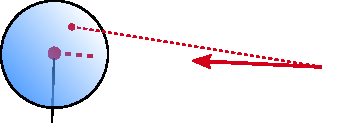
\includegraphics[width=\unitlength,page=1]{waveoptics/scheme/fig1.pdf}}%
    \put(0.60751925,0.11664896){\makebox(0,0)[lt]{\lineheight{1.25}\smash{\begin{tabular}[!ht]{l}$\hatbfR_{ij}$\end{tabular}}}}%
    \put(0.16062109,0.32816852){\makebox(0,0)[lt]{\lineheight{1.25}\smash{\begin{tabular}[!ht]{l}$\bfr$\end{tabular}}}}%
    \put(0.07421882,0.24728563){\makebox(0,0)[lt]{\lineheight{1.25}\smash{\begin{tabular}[!ht]{l}$\bfR_i$\end{tabular}}}}%
    \put(0,0){\includegraphics[width=\unitlength,page=2]{waveoptics/scheme/fig1.pdf}}%
    \put(0.89705938,0.21499518){\makebox(0,0)[lt]{\lineheight{1.25}\smash{\begin{tabular}[!ht]{l}$\bfR_j$\end{tabular}}}}%
    \put(0.44482242,-0.03488032){\makebox(0,0)[lt]{\lineheight{1.25}\smash{\begin{tabular}[!ht]{l}$R_{ij}$\end{tabular}}}}%
    \put(0.02900386,0.14771827){\makebox(0,0)[lt]{\lineheight{1.25}\smash{\begin{tabular}[!ht]{l}$V_i$\end{tabular}}}}%
    \put(0.83481314,0.11979532){\makebox(0,0)[lt]{\lineheight{1.25}\smash{\begin{tabular}[!ht]{l}$V_j$\end{tabular}}}}%
    \put(0,0){\includegraphics[width=\unitlength,page=3]{waveoptics/scheme/fig1.pdf}}%
  \end{picture}%
\endgroup%
 \\ [8pt]  
	\textbf{(a)} \\
	\def\svgwidth{.5\textwidth}
	%% Creator: Inkscape 1.0.2 (e86c870879, 2021-01-15, custom), www.inkscape.org
%% PDF/EPS/PS + LaTeX output extension by Johan Engelen, 2010
%% Accompanies image file 'fig2.pdf' (pdf, eps, ps)
%%
%% To include the image in your LaTeX document, write
%%   \input{<filename>.pdf_tex}
%%  instead of
%%   \includegraphics{<filename>.pdf}
%% To scale the image, write
%%   \def\svgwidth{<desired width>}
%%   \input{<filename>.pdf_tex}
%%  instead of
%%   \includegraphics[width=<desired width>]{<filename>.pdf}
%%
%% Images with a different path to the parent latex file can
%% be accessed with the `import' package (which may need to be
%% installed) using
%%   \usepackage{import}
%% in the preamble, and then including the image with
%%   \import{<path to file>}{<filename>.pdf_tex}
%% Alternatively, one can specify
%%   \graphicspath{{<path to file>/}}
%% 
%% For more information, please see info/svg-inkscape on CTAN:
%%   http://tug.ctan.org/tex-archive/info/svg-inkscape
%%
\begingroup%
  \makeatletter%
  \providecommand\color[2][]{%
    \errmessage{(Inkscape) Color is used for the text in Inkscape, but the package 'color.sty' is not loaded}%
    \renewcommand\color[2][]{}%
  }%
  \providecommand\transparent[1]{%
    \errmessage{(Inkscape) Transparency is used (non-zero) for the text in Inkscape, but the package 'transparent.sty' is not loaded}%
    \renewcommand\transparent[1]{}%
  }%
  \providecommand\rotatebox[2]{#2}%
  \newcommand*\fsize{\dimexpr\f@size pt\relax}%
  \newcommand*\lineheight[1]{\fontsize{\fsize}{#1\fsize}\selectfont}%
  \ifx\svgwidth\undefined%
    \setlength{\unitlength}{195.27076845bp}%
    \ifx\svgscale\undefined%
      \relax%
    \else%
      \setlength{\unitlength}{\unitlength * \real{\svgscale}}%
    \fi%
  \else%
    \setlength{\unitlength}{\svgwidth}%
  \fi%
  \global\let\svgwidth\undefined%
  \global\let\svgscale\undefined%
  \makeatother%
  \begin{picture}(1,0.5215872)%
    \lineheight{1}%
    \setlength\tabcolsep{0pt}%
    \put(0,0){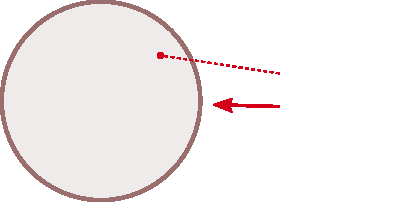
\includegraphics[width=\unitlength,page=1]{waveoptics/scheme/fig2.pdf}}%
    \put(0.92645221,0.21560272){\makebox(0,0)[lt]{\lineheight{1.25}\smash{\begin{tabular}[t]{l}$\bfR_k$\end{tabular}}}}%
    \put(0.56274836,0.21221995){\makebox(0,0)[lt]{\lineheight{1.25}\smash{\begin{tabular}[t]{l}$\hatbfR_{\Cls k}$\end{tabular}}}}%
    \put(0.33172694,0.34184498){\makebox(0,0)[lt]{\lineheight{1.25}\smash{\begin{tabular}[t]{l}$\bfR_i$\end{tabular}}}}%
    \put(0.15998663,0.24282036){\makebox(0,0)[lt]{\lineheight{1.25}\smash{\begin{tabular}[t]{l}$\bfR_\Cls$\end{tabular}}}}%
    \put(0,0){\includegraphics[width=\unitlength,page=2]{waveoptics/scheme/fig2.pdf}}%
    \put(0.47642379,0.08204267){\makebox(0,0)[lt]{\lineheight{1.25}\smash{\begin{tabular}[t]{l}$R_{\Cls k}$\end{tabular}}}}%
    \put(0,0){\includegraphics[width=\unitlength,page=3]{waveoptics/scheme/fig2.pdf}}%
    \put(0.59047783,0.30130627){\makebox(0,0)[lt]{\lineheight{1.25}\smash{\begin{tabular}[t]{l}$\hatbfR_{ik}$\end{tabular}}}}%
    \put(0.07747599,0.39359056){\makebox(0,0)[lt]{\lineheight{1.25}\smash{\begin{tabular}[t]{l}$\Cls$\end{tabular}}}}%
    \put(0,0){\includegraphics[width=\unitlength,page=4]{waveoptics/scheme/fig2.pdf}}%
  \end{picture}%
\endgroup%
 \\ [-5pt]
	\textbf{(b)} \\ [5pt]
	\def\svgwidth{.5\textwidth}
	%% Creator: Inkscape 1.0.2 (e86c870879, 2021-01-15, custom), www.inkscape.org
%% PDF/EPS/PS + LaTeX output extension by Johan Engelen, 2010
%% Accompanies image file 'fig3.pdf' (pdf, eps, ps)
%%
%% To include the image in your LaTeX document, write
%%   \input{<filename>.pdf_tex}
%%  instead of
%%   \includegraphics{<filename>.pdf}
%% To scale the image, write
%%   \def\svgwidth{<desired width>}
%%   \input{<filename>.pdf_tex}
%%  instead of
%%   \includegraphics[width=<desired width>]{<filename>.pdf}
%%
%% Images with a different path to the parent latex file can
%% be accessed with the `import' package (which may need to be
%% installed) using
%%   \usepackage{import}
%% in the preamble, and then including the image with
%%   \import{<path to file>}{<filename>.pdf_tex}
%% Alternatively, one can specify
%%   \graphicspath{{<path to file>/}}
%% 
%% For more information, please see info/svg-inkscape on CTAN:
%%   http://tug.ctan.org/tex-archive/info/svg-inkscape
%%
\begingroup%
  \makeatletter%
  \providecommand\color[2][]{%
    \errmessage{(Inkscape) Color is used for the text in Inkscape, but the package 'color.sty' is not loaded}%
    \renewcommand\color[2][]{}%
  }%
  \providecommand\transparent[1]{%
    \errmessage{(Inkscape) Transparency is used (non-zero) for the text in Inkscape, but the package 'transparent.sty' is not loaded}%
    \renewcommand\transparent[1]{}%
  }%
  \providecommand\rotatebox[2]{#2}%
  \newcommand*\fsize{\dimexpr\f@size pt\relax}%
  \newcommand*\lineheight[1]{\fontsize{\fsize}{#1\fsize}\selectfont}%
  \ifx\svgwidth\undefined%
    \setlength{\unitlength}{229.25272174bp}%
    \ifx\svgscale\undefined%
      \relax%
    \else%
      \setlength{\unitlength}{\unitlength * \real{\svgscale}}%
    \fi%
  \else%
    \setlength{\unitlength}{\svgwidth}%
  \fi%
  \global\let\svgwidth\undefined%
  \global\let\svgscale\undefined%
  \makeatother%
  \begin{picture}(1,0.74203056)%
    \lineheight{1}%
    \setlength\tabcolsep{0pt}%
    \put(0,0){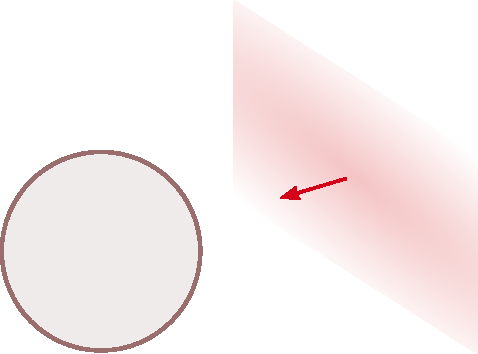
\includegraphics[width=\unitlength,page=1]{waveoptics/scheme/fig3.pdf}}%
    \put(0.65700635,0.28170623){\makebox(0,0)[lt]{\lineheight{1.25}\smash{\begin{tabular}[t]{l}$\hatbfR_{\Cls k}$\end{tabular}}}}%
    \put(0.12349537,0.189373){\makebox(0,0)[lt]{\lineheight{1.25}\smash{\begin{tabular}[t]{l}$\bfR_\Cls$\end{tabular}}}}%
    \put(0,0){\includegraphics[width=\unitlength,page=2]{waveoptics/scheme/fig3.pdf}}%
    \put(0.05895636,0.31779465){\makebox(0,0)[lt]{\lineheight{1.25}\smash{\begin{tabular}[t]{l}$\Cls$\end{tabular}}}}%
    \put(0,0){\includegraphics[width=\unitlength,page=3]{waveoptics/scheme/fig3.pdf}}%
    \put(0.49113417,0.59209251){\makebox(0,0)[lt]{\lineheight{1.25}\smash{\begin{tabular}[t]{l}$\bfEe_{\Cls k}$\end{tabular}}}}%
    \put(0.73597331,0.45319112){\makebox(0,0)[lt]{\lineheight{1.25}\smash{\begin{tabular}[t]{l}$\theta^{\text{inc}}$\end{tabular}}}}%
    \put(0.78775278,0.33127162){\makebox(0,0)[lt]{\lineheight{1.25}\smash{\begin{tabular}[t]{l}$\phi^{\text{inc}}$\end{tabular}}}}%
  \end{picture}%
\endgroup%
 \\ [-5pt]
	\textbf{(c)}
	
	\caption[Schematical representation of the particles scattering geometry]{\label{fig:waveoptics:diagram}
	  	\textbf{Schematical representation of the particles scattering geometry.} \textbf{(a)} Previous methods, including Lorenz-Mie theory, assume independent scattering of particles, assuming that the distance $R_{ij}$ between two particles $i$ and $j$ is very large (i.e. $R_{ij}\rightarrow\infty$), neglecting the potential interactions between particles. \textbf{(b)} In our work  we differentiate between near field scattering of particles within a small region in space (cluster $\Cls$ centered at $\bfR_\Cls$), and particles $k$ on the far-field region of the cluster (distance $R_{\Cls k}\rightarrow\infty$). \textbf{(c)} For large values of $R_{\Cls k}$, the direction between particle $k$ and any particle $j\in\Cls$ is $dPx_{ik}\approx\hatbfR_{\Cls k}$: Therefore, we can assume an planar exciting field $\bfEe(\bfr)_{\Cls k}$ on the whole cluster $\Cls$ from particle $k$, with direction $\hatbfR_{\Cls k}$. 
	}
\end{figure}

\paragraph{Far-field Foldy-Lax Equations}
\Eq{eq:excfield} defines the exact exciting field resulting from the scattering by particle~$j$ on particle~$i$.
However, if the distance $\tPx_{ij} \defeq \| \Px_i - \Px_j \|$ between particles (with $\Px_i$ denoting the center of particle $i$) is large, we can approximate the propagation distance between any point $\px \in V_i$ and $\px' \in V_j$ as
\begin{equation}
    \| \px - \px' \| \approx \tPx_{ij} + (\dPx_{ij} \cdot {\Delta}\px) -  (\dPx_{ij} \cdot {\Delta}\px'),
\end{equation}
with $\dPx_{ij} \defeq (\Px_i - \Px_j)/\tPx_{ij}$, ${\Delta}\px \defeq \px - \Px_i$ and ${\Delta}\px' \defeq \px' - \Px_j$ (see Figure \ref{fig:waveoptics:diagram}, left).
With this approximation, we can now express $\ExcEField_{ij}(\px)$ for a point $\px \in V_i$ using its \emph{far-field} approximation, as:%
\footnote{We note that, accordingly to Mishchenko \cite{mishchenko2006multiple}, the product would require to multiply the integrand by the dyad $(\sIdDyad - \dPx_{ij}\otimes\dPx_{ij})$ to ensure a transverse planar field; we remove it for clarity.}
\begin{equation}
    \begin{split}
        & \ExcEField_{ij}(\px)\\
        \approx\;& \frac{\E^{\img k_1 (\tPx_{ij}+\dPx_{ij}\cdot{\Delta}\px)}}{4\pi\tPx_{ij}} \int_{V_j} \sGreenProp(\dPx_{ij},{\Delta}\px') \int_{V_j} \dyad{T}_j(\px',\px'')\cdot \EField_j(\px'') \diff{\px''}\,\diff{\px'} \\
        =\;& \frac{\exp(\img k_1 \,\tPx_{ij})}{\tPx_{ij}} 
        \sGreenProp(\dPx_{ij}, \Delta \px) \,\ExcEField_{1ij}(\dPx_{ij}),
    \end{split}
    \label{eq:excfieldfar}
    \raisetag{17pt}
\end{equation}
where: $\px \in V_i$ is a point in particle $i$; $\sGreenProp(\dw, \Delta \px)=\exp(\img k_1 \,\dPx_{ij}\cdot{\Delta}\px)$; and $\ExcEField_{1ij}$ is the far-field exciting field from particle $j$ to particle $i$ that is solely characterized by the propagation direction $\dPx_{ij}$. In order for \Eq{eq:excfieldfar} to be valid, the distance $\tPx_{ij}$ needs to hold the far-field criteria, which relates the $\tPx_{ij}$ with the radius of the particle $\radius_j$ following the inequality~\cite{mishchenko2006multiple}:
\begin{equation}
    k_1 \tPx_{ij} \gg \max\left(1, \frac{k_1^2\radius_j^2}{2}\right).
    \label{eq:farfield}
\end{equation}
This far-field assumption is both the basis for the Lorenz-Mie theory \cite{hulst1981light} (to model electromagnetic scattering from small spherical particles) and, as shown by Mishchenko \cite{mishchenko2002vector}, at the core of the radiative transfer theory.

In the following, we relax the assumption of near field scattering and compute the Foldy-Lax equations for clusters of particles for both the near- and far-field regions. Then, we use them to compute the scattering matrix to be used in the RTE to efficiently approximate light transport between clusters of particles. 
